\section{Evaluation of a traceability solution: Capra}\label{sec:evaluationcapra}
\sideboxbegin{o}
This section depicts how the protocol from Section \ref{sec:protocol-evaluation} has been applied to evaluate Capra. The adaptativeness of the tool through customization and visualization features is put forward ; identification and quality assessment remain slightly back.
\sideboxend



Capra is a promising generic solution to model-based software traceability \cite{heisig2019-generic-traceability-metamodel-end-to-end-capra,maro2016_maintenance_factors_and_guidelines}. Yet, as we will see, it suffers an obvious lack of means to consider the quality of traces.
In this section, after a brief introduction to Capra, we detail the application of the protocol introduced in Section \ref{sec:protocol-evaluation} on that specific solution. We detail each of the five steps and summarize the results in Table \ref{tab:evaluationcapra} to establish whether, or to what cost, Capra would fit a consequent industrial exploitation.

\begin{descriptioncompact}
    \item[Quick presentation of Capra] Capra is a tool and a research project aiming at generic software traceability \cite{heisig2019-generic-traceability-metamodel-end-to-end-capra,maro2016_maintenance_factors_and_guidelines}. Its initiators rose the ability to trace as a noticeably important feature to integrate into the realm of model-driven engineering \cite{hotlmann2020-MB-traceability-terminology}. Scientific publications show that strong traceability has been long due in the field and Capra's authors distinguish themselves from other approaches with an important focus on customizability and visualization of tracing artefacts \cite{clelandhuang2007bestPracticeForAutomatedTraceability,mader2010-visual-tracability-modeling-language}. The overall goal of Capra is to allow the linking of elements from different domain specific modeling languages.

    \begin{figure}[h]  
    	\centering
    	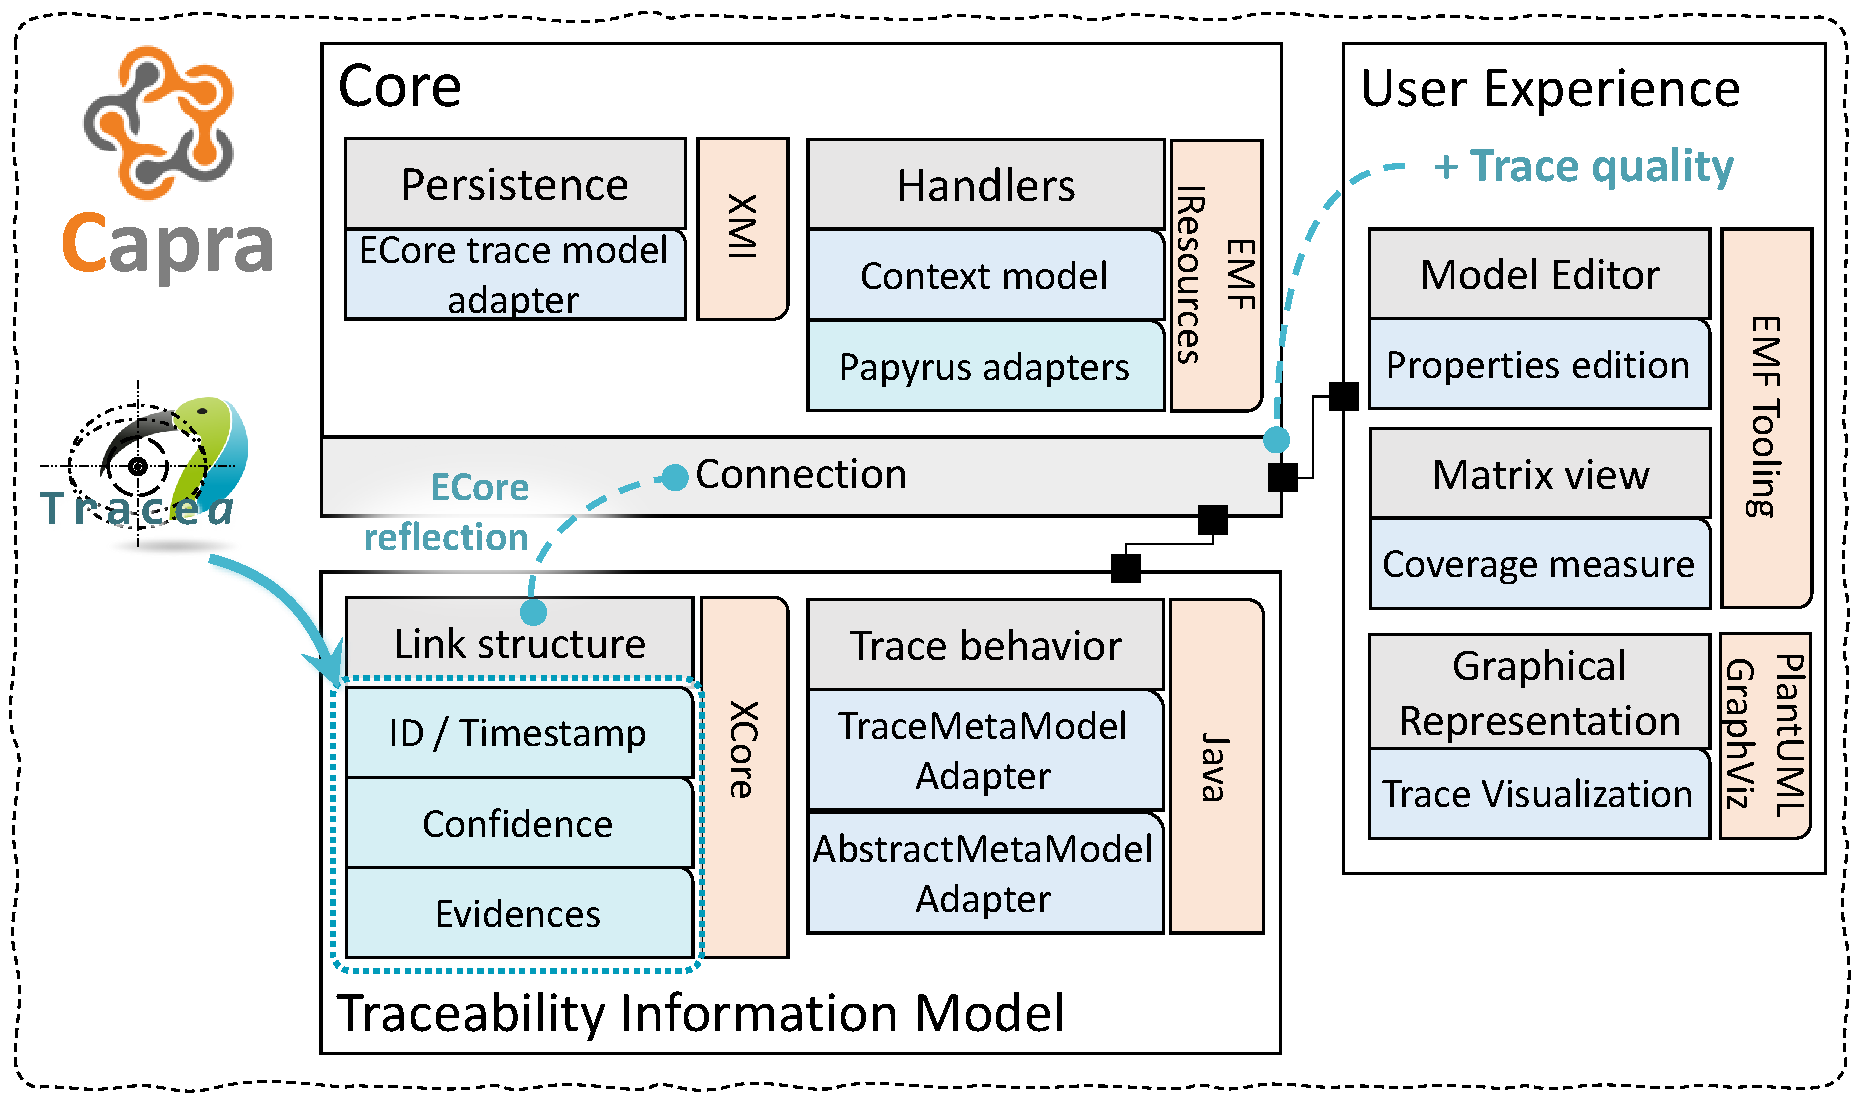
\includegraphics[width=.85\linewidth]{images/capra-architecture}
    	\caption{Architecture of Capra}
    	\label{fig:capraarchitecture}
    \end{figure}
    
    See \Fig{fig:capraarchitecture} for a detailed view of Capra architecture. The implementation of the tracer is based on the Eclipse Modeling Framework \cite{EMF} hosted open on Git \cite{Capra_Repo}. It consists of an Eclipse plugin that carries out the requirements an industrial partner mandates.  There is a core package, which grows into new handlers to support more and more domain specific languages and usages\footnote{To quote but one example, Capra is ready to use with Papyrus models and elements.}. A package is dedicated to the customization of the traceability information model (or trace model), and the UI is based on Eclipse's ECore model editor and PlantUML for diagrammatic representations.
     
    The maintenance of the tool is ensured mainly by the authors of the publications. They are quick to answer questions and comments.
    
    

\end{descriptioncompact}


\subsection{Traceability customization}\label{sec:custom}

Capra allows a custom definition of the artefacts' and relationships' types. The customization of artefacts and links is editable through an XCore plugin\footnote{More details can be found at: \url{https://wiki.eclipse.org/Capra/CustomTraceabilityMetaModel}}. Links can be defined following a hierarchical inheritance and allowing structural features (reference and attributes)\footnote{There is no guaranty on the level of implementation of the more complex features XCore allows.}. 

Capra is an EMF plugin and benefits from the artefacts used by the running instance of the platform. An artefact is defined through the resource change management plugin mechanism of EMF infrastructure. The wrapping of the artefacts uses another XCore plugin. It allows the definition of other attributes for artefacts: \verb|org.eclipse.capra.generic.artefactmodel|.
The adapters, handlers, and helpers for the EMF artefacts must be redefined as Java polymorphic overriding projects (derived from \verb|org.eclipse.capra.generic.core|).  
Capra redefines wrappers for 15 languages or standards such as UML, BPMN, Papyrus, Mylyn, Java, C++ Office, to name a few\footnote{There is no documentation relating the means to apply such redefinition - neither can be found any tips on the potential impact such changes may initiate.}. 

By default there is one generic \textit{RelatedTo} possible kind of link. For each link, there must be one and only one source and one or more target artefacts (target cardinality can be changed). The types of origin and target artefacts can be constrained.

In the default implementation, links are part of a \texttt{TraceModel} that \textit{connects} between them. There is no explicit trace structure but a \textit{behavior} defined in Java. 
If an artefact is part of the target of a link and the origin of another, the trace connects (see the Section \ref{sec:visualization} on visualization). This implementation (\verb|org.eclipse.capra.generic.GenericTraceModel|) must be transferred or adapted (Java file, no documentation) to be adapted to a new structure. There is no test coverage for potential alterations to the original implementation. 

\subsection{Links identification}\label{sec:identification}
Identifying links in Capra is done manually. Any element actionable in an Eclipse environment can be selected to take part of a trace. A context menu reacts to elements and offers to add to the "Traceability selection", or drag-n-drop the element into the \texttt{Trace Creation}\footnote{Names are subject to change.} view (\Fig{fig:tracecreation}). (Respective adapters are required, see Section \ref{sec:custom}.)
There is no automation for the identification of relationships, but the UML dependencies can be viewed in the \texttt{Capra PlantUML Viewer}. UML relations are not part of the serialized of the trace links. They are derived for (visual) convenience and they need to be manually recorded to be serialized.

\begin{figure}[h] 
	\centering
	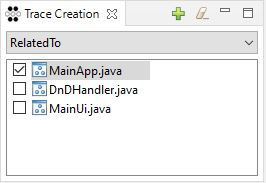
\includegraphics[width=.35\linewidth]{images/tracecreationview.JPG}
	\caption{Capra's Trace Creation view}
	\label{fig:tracecreation}
\end{figure}

\subsection{Trace visualization \& Retrieval}\label{sec:visualization}
Capra's prime feature is a multi-paradigm visualization support with textual, graphical and matrix representations. 
The second, based on PlantUML/Graphviz, supports developers in change impact analysis ; the matrix representation facilitates the evaluation of test coverage. Mixing the two allows an in depth safety analysis - Capra's authors next publication will show this last point\footnote{From an interview with the main Git contributor and author.}. 
	
\begin{descriptioncompact}
    \item[Augmented text representation of links] 
Traces in Capra are serialized into XMI Ecore models. This is convenient since Eclipse offers a \texttt{Reflexive Ecore Model Editor} to browse and edit such resources. Traces themselves cannot be apprehended though, if not to a great cost, because this view does not show the succession of trace links. \Fig{fig:xmieditor} shows a screenshot of this view. As can be seen, a name composed with the name of the artefacts targeted is the only information available - together with the elements properties in the \texttt{Properties} view associated. 
Instances of the wrappers for the artefacts used by the trace links are stored in the same manner in another XMI file.
\begin{figure}[h] 
	\centering
	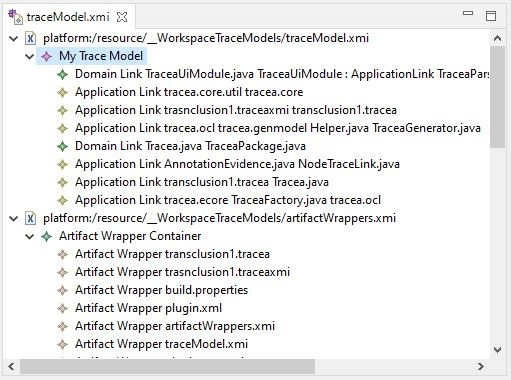
\includegraphics[width=.65\linewidth]{images/XMIEditor.jpg}
	\caption{Links and artefact wrappers, browsed with Eclipse Ecore Model editor}
	\label{fig:xmieditor}
\end{figure}

    \item[Graphical representation of traces] %using PlantUML/GraphViz plugin
To ease the visualization, Capra generates a graphical description of traces in GraphViz\footnote{\url{https://graphviz.org/}} and uses PlantUML\footnote{\url{https://plantuml.com/}} to plot them in an Eclipse view. Figure \ref{fig:plantuml} shows a capture of the view.
This view shows the links associated to the element selected in the Eclipse IDE. These links are the one {identified} with Capra (the trace links) or are derived from the neighborhood of the element selected. In the case of a Java class, a type hierarchy is provided.
The view is configurable. The type of links, as well as {the depth of transitivity} can be changed through the Eclipse interface.  
\begin{figure}[h] 
	\centering
	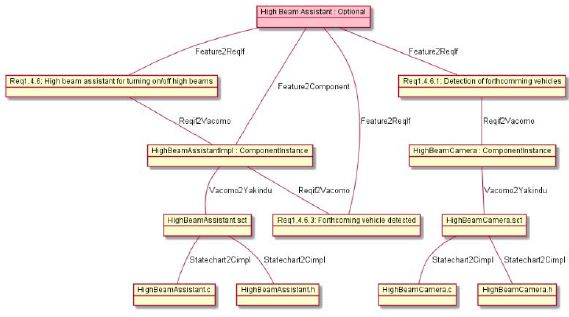
\includegraphics[width=.60\linewidth]{images/plantuml-viewer.jpg}
	\caption{Trace links sequences are plotted graphically in Capra PlantUML Viewer}
	\label{fig:plantuml}
\end{figure}

    \item[Matrix-based representation of tracing] 
%Numerous authors in traceability shows the importance of a \ughu{broader} point of view on the tracing process that shows the linkage between the traced artefacts through an association matrix. 
Capra offers an association matrix view, as can be seen in \Fig{fig:matrixviewer}. This view shows links from a high-level perspective and is most useful for coverage measurement. It can be exported in the Excel (xls) format.
\begin{figure}[h] 
	\centering
	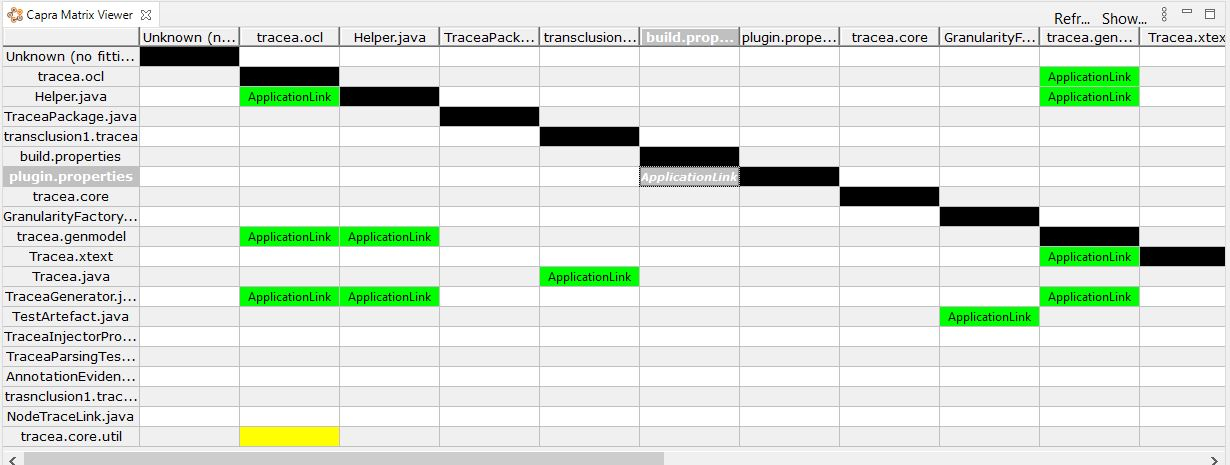
\includegraphics[width=.65\linewidth]{images/matrixViewer.jpg}
	\caption{Interrelations can be viewed in the matrix-based representation}
	\label{fig:matrixviewer}
\end{figure}

    \item[Link retrieval] There is no mechanism to retrieve automatically trace links. Yet, the use of Viatra-IncQuery\footnote{\url{https://www.eclipse.org/viatra/}} is a strong bet to address this limitation for it is tailored to XMI Ecore resources and offers many features for querying and generating Ecore models.
\end{descriptioncompact}


\subsection{Trace persistence \& Edition}
\begin{figure}[h] 
	\centering
	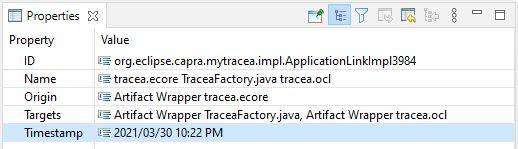
\includegraphics[width=.65\linewidth]{images/properties.jpg}
	\caption{Links are viewed and edited with Eclipse Properties view}
	\label{fig:properties}
\end{figure}
Traces are serialized into an Ecore model, stored in an XMI file. Artefacts wrappers are also stored in XMI.
The \texttt{Reflexive Ecore Model Editor} (together with the \texttt{Properties} view, see  \Fig{fig:properties}) can be used to edit the information but \textbf{the consistency of other views is not guarantied.} Eclipse must be closed and reopened.
The name of the files appear in the project list, but their name cannot be edited. 
\textbf{It is highly recommended to not modify the files, nor delete them.} The default \texttt{PlantUML viewer} does not offers any means to interact with the trace.


\subsection{Trace quality evaluation}
Capra checks the consistency of traces when artefacts are modified or deleted through the Eclipse platform. Changes in the software elements triggers a validity check on the links these elements take part in (as source or target). As a consequence, the links are tagged with a warning. There is no fix proposed.

Confidence is not quantified and there is no record of the facts or evidences about the existence of a link.

\subsection{Conclusion}

Table \ref{tab:evaluationcapra} summarizes the evaluation of Capra, and \Fig{fig:evaluationcapra} illustrates the summary with regard to the traceability infrastructure overview. As can be seen, the tool benefits a strong customization potential. On the one hand, it is easy to design wrappers for new artefacts with Eclipse \texttt{IResource} redefinition, and the definition of link types is very expressive thanks to XCore.   
On the other hand, if the tool lacks some automated mechanisms to identify traces, the visualization of both specific links and derived UML relations is very powerful. 
Capra is currently used in three use cases: Change Impact Analysis, Coverage analysis, and Safety analysis, with a publication to come on these matters. 

On a bad note, the absence of means to edit safely trace links is a major impediment to the use of Capra in an industrial context. Discussing with the authors on the matter showed there is no plan to address this issue. They do not consider the use of the XMI editor as a convenient mean to edit traces.

The tool also suffers a lack of trace quality assessment. 
There is one feature related to quality in Capra which consists in a consistency check that triggers warnings when resources targeted by traces are modified or deleted in the Eclipse environment.
Yet, there is no evaluation of any kind of confidence level and less explainability resources. This is a recurrent limitations that most if not all traceability solutions suffer~\cite{batot2020-survey-driven-feature-model,batot2021-not-another-metamodel}. 


As a conclusion, Capra is a rather good tool for traceability in terms of adaptativeness -- and that is a very important concern to tracer design. The quality of trace links is not considered, as expected -- but we show in the next section how to extend Capra with Trace\textit{a} to circumcise this limitation.

\begin{table}[h]   
	\centering
	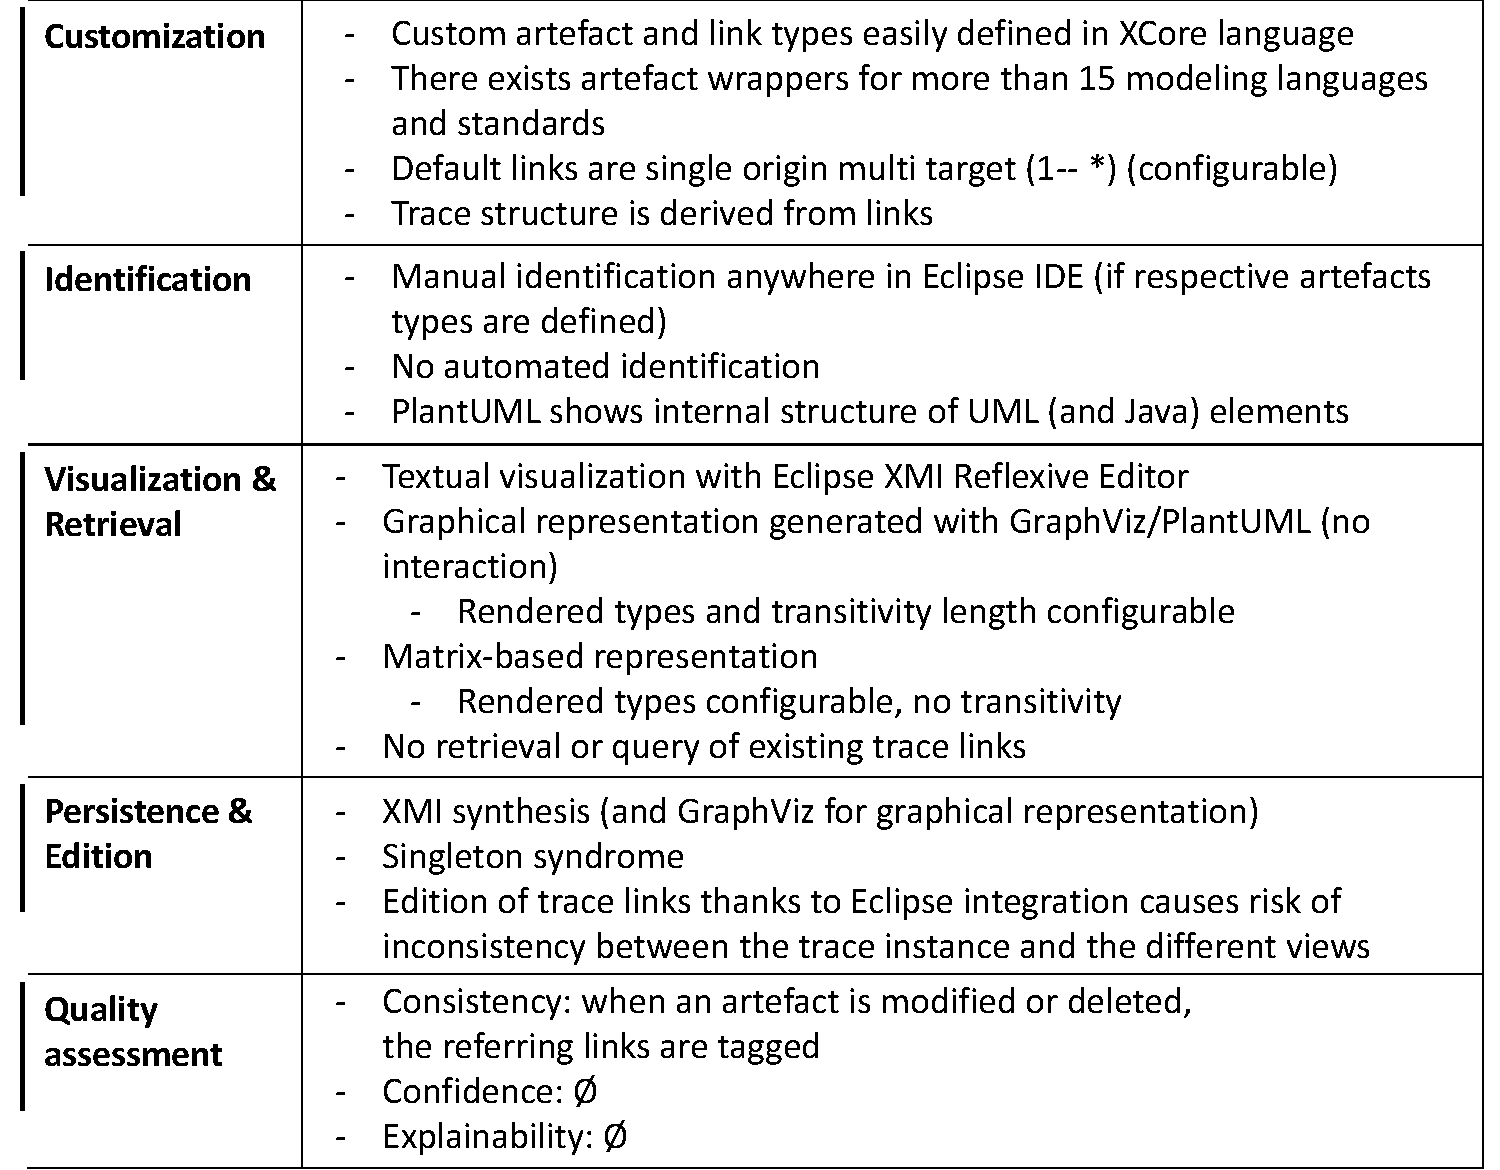
\includegraphics[width=.85\linewidth]{images/evaluation-table-capra.pdf}
	\caption{Summary of the evaluation of Capra}
	\label{tab:evaluationcapra}
\end{table}
\begin{figure}[h]  
	\centering
	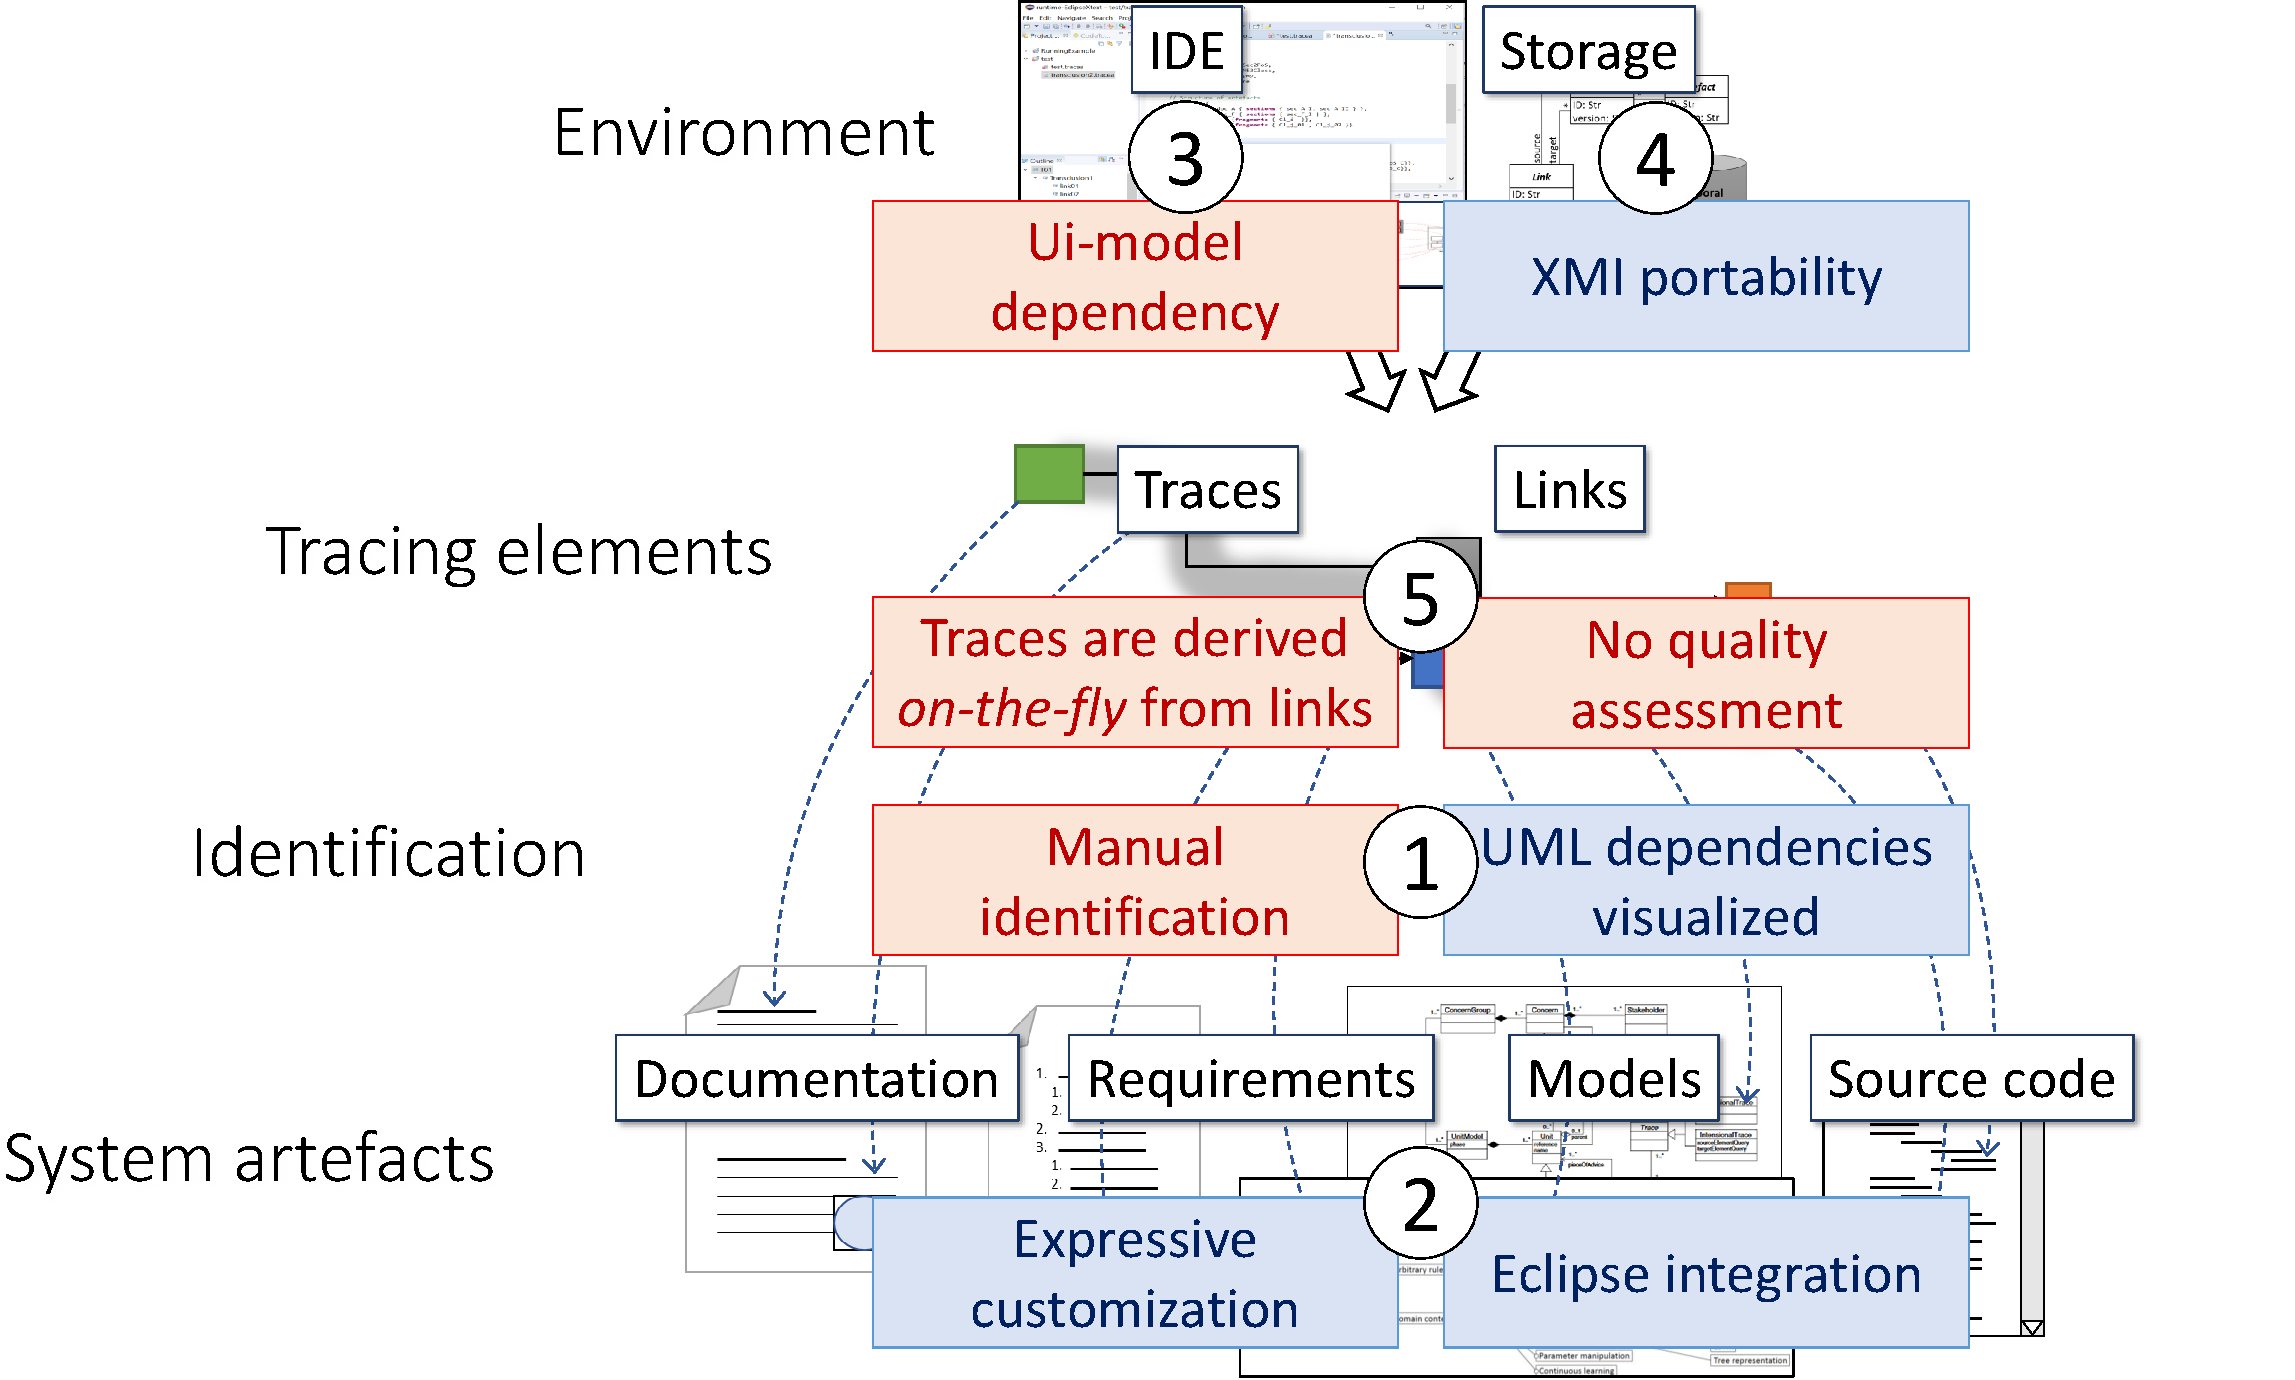
\includegraphics[width=.7\linewidth]{images/evaluation-points-capra.pdf}
	\caption{Summary of the evaluation of Capra}
	\label{fig:evaluationcapra}
\end{figure}

